\documentclass[1p]{elsarticle_modified}
%\bibliographystyle{elsarticle-num}

%\usepackage[colorlinks]{hyperref}
%\usepackage{abbrmath_seonhwa} %\Abb, \Ascr, \Acal ,\Abf, \Afrak
\usepackage{amsfonts}
\usepackage{amssymb}
\usepackage{amsmath}
\usepackage{amsthm}
\usepackage{scalefnt}
\usepackage{amsbsy}
\usepackage{kotex}
\usepackage{caption}
\usepackage{subfig}
\usepackage{color}
\usepackage{graphicx}
\usepackage{xcolor} %% white, black, red, green, blue, cyan, magenta, yellow
\usepackage{float}
\usepackage{setspace}
\usepackage{hyperref}

\usepackage{tikz}
\usetikzlibrary{arrows}

\usepackage{multirow}
\usepackage{array} % fixed length table
\usepackage{hhline}

%%%%%%%%%%%%%%%%%%%%%
\makeatletter
\renewcommand*\env@matrix[1][\arraystretch]{%
	\edef\arraystretch{#1}%
	\hskip -\arraycolsep
	\let\@ifnextchar\new@ifnextchar
	\array{*\c@MaxMatrixCols c}}
\makeatother %https://tex.stackexchange.com/questions/14071/how-can-i-increase-the-line-spacing-in-a-matrix
%%%%%%%%%%%%%%%

\usepackage[normalem]{ulem}

\newcommand{\msout}[1]{\ifmmode\text{\sout{\ensuremath{#1}}}\else\sout{#1}\fi}
%SOURCE: \msout is \stkout macro in https://tex.stackexchange.com/questions/20609/strikeout-in-math-mode

\newcommand{\cancel}[1]{
	\ifmmode
	{\color{red}\msout{#1}}
	\else
	{\color{red}\sout{#1}}
	\fi
}

\newcommand{\add}[1]{
	{\color{blue}\uwave{#1}}
}

\newcommand{\replace}[2]{
	\ifmmode
	{\color{red}\msout{#1}}{\color{blue}\uwave{#2}}
	\else
	{\color{red}\sout{#1}}{\color{blue}\uwave{#2}}
	\fi
}

\newcommand{\Sol}{\mathcal{S}} %segment
\newcommand{\D}{D} %diagram
\newcommand{\A}{\mathcal{A}} %arc


%%%%%%%%%%%%%%%%%%%%%%%%%%%%%5 test

\def\sl{\operatorname{\textup{SL}}(2,\Cbb)}
\def\psl{\operatorname{\textup{PSL}}(2,\Cbb)}
\def\quan{\mkern 1mu \triangleright \mkern 1mu}

\theoremstyle{definition}
\newtheorem{thm}{Theorem}[section]
\newtheorem{prop}[thm]{Proposition}
\newtheorem{lem}[thm]{Lemma}
\newtheorem{ques}[thm]{Question}
\newtheorem{cor}[thm]{Corollary}
\newtheorem{defn}[thm]{Definition}
\newtheorem{exam}[thm]{Example}
\newtheorem{rmk}[thm]{Remark}
\newtheorem{alg}[thm]{Algorithm}

\newcommand{\I}{\sqrt{-1}}
\begin{document}

%\begin{frontmatter}
%
%\title{Boundary parabolic representations of knots up to 8 crossings}
%
%%% Group authors per affiliation:
%\author{Yunhi Cho} 
%\address{Department of Mathematics, University of Seoul, Seoul, Korea}
%\ead{yhcho@uos.ac.kr}
%
%
%\author{Seonhwa Kim} %\fnref{s_kim}}
%\address{Center for Geometry and Physics, Institute for Basic Science, Pohang, 37673, Korea}
%\ead{ryeona17@ibs.re.kr}
%
%\author{Hyuk Kim}
%\address{Department of Mathematical Sciences, Seoul National University, Seoul 08826, Korea}
%\ead{hyukkim@snu.ac.kr}
%
%\author{Seokbeom Yoon}
%\address{Department of Mathematical Sciences, Seoul National University, Seoul, 08826,  Korea}
%\ead{sbyoon15@snu.ac.kr}
%
%\begin{abstract}
%We find all boundary parabolic representation of knots up to 8 crossings.
%
%\end{abstract}
%\begin{keyword}
%    \MSC[2010] 57M25 
%\end{keyword}
%
%\end{frontmatter}

%\linenumbers
%\tableofcontents
%
\newcommand\colored[1]{\textcolor{white}{\rule[-0.35ex]{0.8em}{1.4ex}}\kern-0.8em\color{red} #1}%
%\newcommand\colored[1]{\textcolor{white}{ #1}\kern-2.17ex	\textcolor{white}{ #1}\kern-1.81ex	\textcolor{white}{ #1}\kern-2.15ex\color{red}#1	}

{\Large $\underline{12a_{0468}~(K12a_{0468})}$}

\setlength{\tabcolsep}{10pt}
\renewcommand{\arraystretch}{1.6}
\vspace{1cm}\begin{tabular}{m{100pt}>{\centering\arraybackslash}m{274pt}}
\multirow{5}{120pt}{
	\centering
	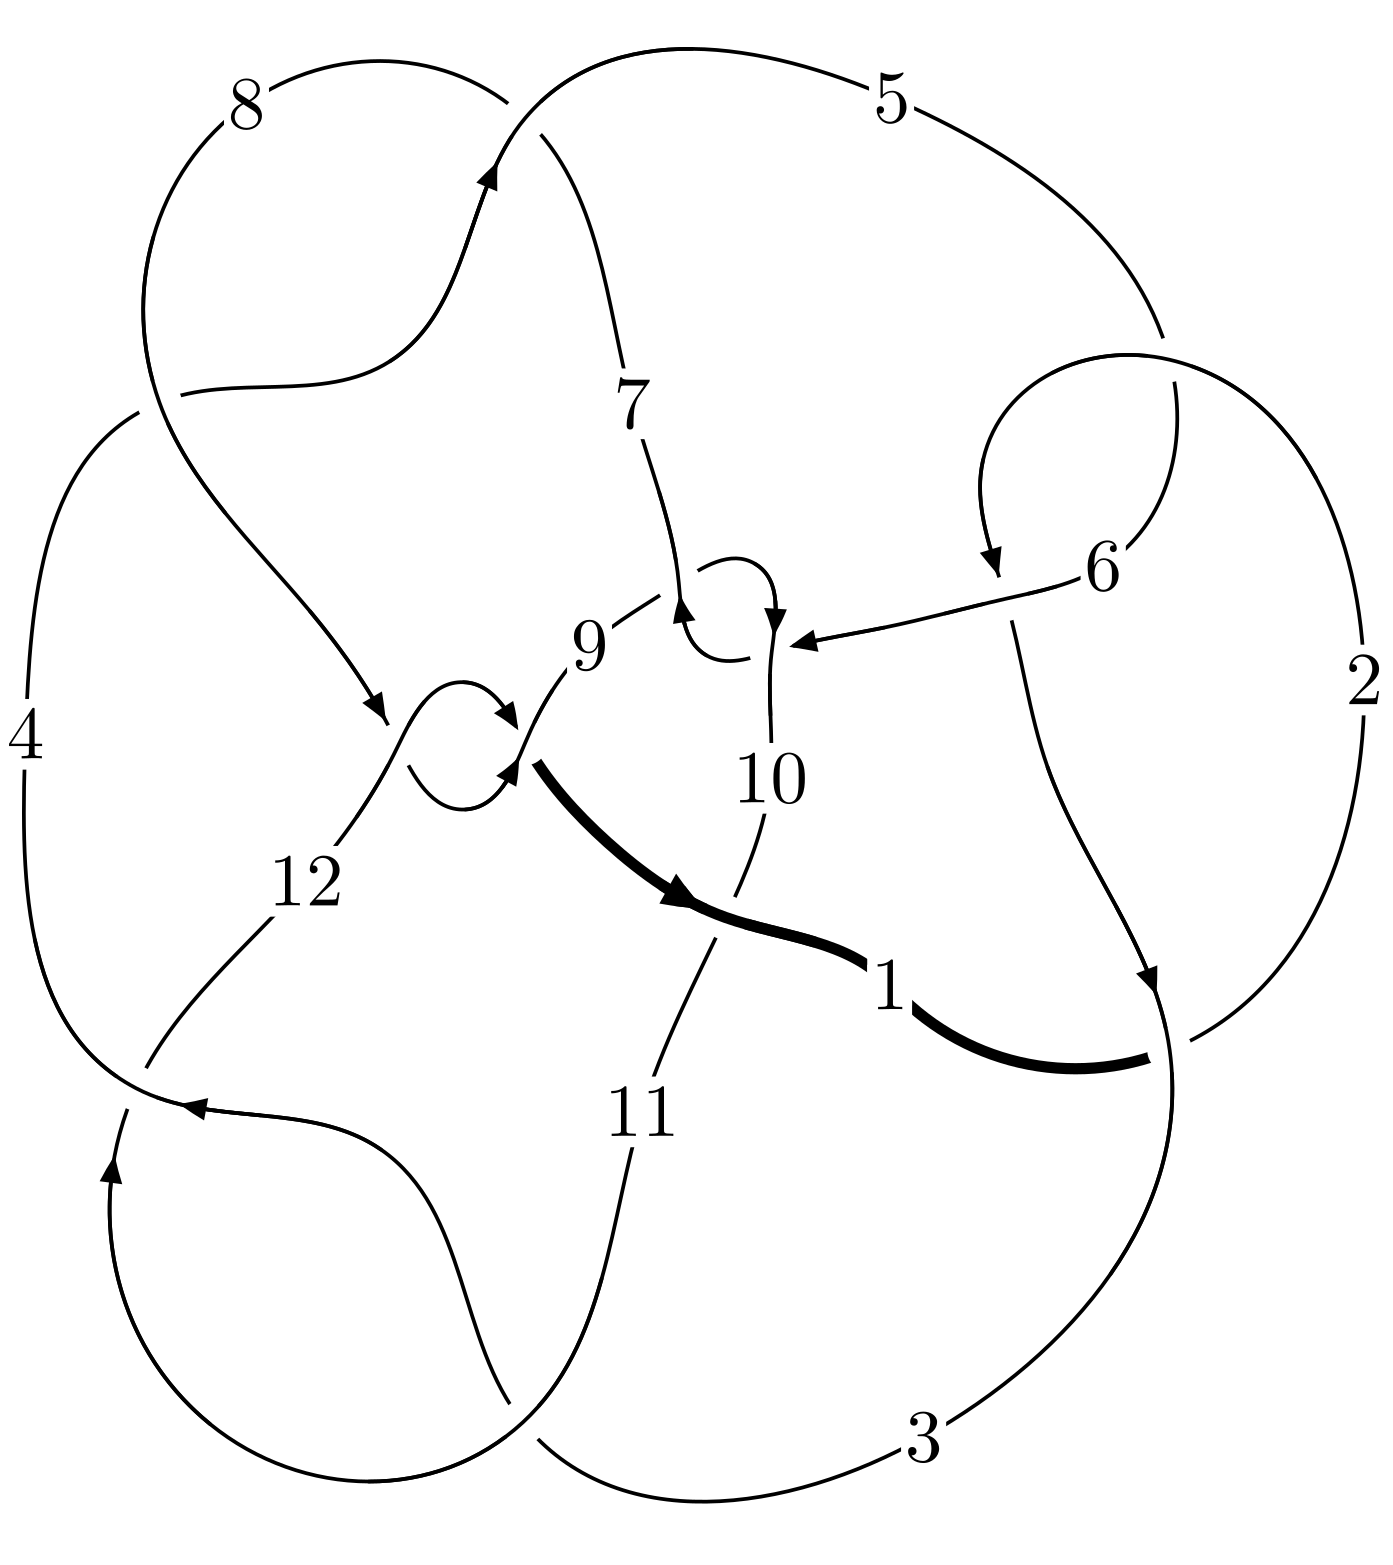
\includegraphics[width=112pt]{../../../GIT/diagram.site/Diagrams/png/1269_12a_0468.png}\\
\ \ \ A knot diagram\footnotemark}&
\allowdisplaybreaks
\textbf{Linearized knot diagam} \\
\cline{2-2}
 &
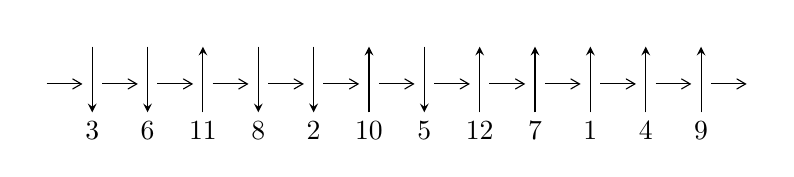
\begin{tikzpicture}[x=20pt, y=17pt]
	% nodes
	\node (C0) at (0, 0) {};
	\node (C1) at (1, 0) {};
	\node (C1U) at (1, +1) {};
	\node (C1D) at (1, -1) {3};

	\node (C2) at (2, 0) {};
	\node (C2U) at (2, +1) {};
	\node (C2D) at (2, -1) {6};

	\node (C3) at (3, 0) {};
	\node (C3U) at (3, +1) {};
	\node (C3D) at (3, -1) {11};

	\node (C4) at (4, 0) {};
	\node (C4U) at (4, +1) {};
	\node (C4D) at (4, -1) {8};

	\node (C5) at (5, 0) {};
	\node (C5U) at (5, +1) {};
	\node (C5D) at (5, -1) {2};

	\node (C6) at (6, 0) {};
	\node (C6U) at (6, +1) {};
	\node (C6D) at (6, -1) {10};

	\node (C7) at (7, 0) {};
	\node (C7U) at (7, +1) {};
	\node (C7D) at (7, -1) {5};

	\node (C8) at (8, 0) {};
	\node (C8U) at (8, +1) {};
	\node (C8D) at (8, -1) {12};

	\node (C9) at (9, 0) {};
	\node (C9U) at (9, +1) {};
	\node (C9D) at (9, -1) {7};

	\node (C10) at (10, 0) {};
	\node (C10U) at (10, +1) {};
	\node (C10D) at (10, -1) {1};

	\node (C11) at (11, 0) {};
	\node (C11U) at (11, +1) {};
	\node (C11D) at (11, -1) {4};

	\node (C12) at (12, 0) {};
	\node (C12U) at (12, +1) {};
	\node (C12D) at (12, -1) {9};
	\node (C13) at (13, 0) {};

	% arrows
	\draw[->,>={angle 60}]
	(C0) edge (C1) (C1) edge (C2) (C2) edge (C3) (C3) edge (C4) (C4) edge (C5) (C5) edge (C6) (C6) edge (C7) (C7) edge (C8) (C8) edge (C9) (C9) edge (C10) (C10) edge (C11) (C11) edge (C12) (C12) edge (C13) ;	\draw[->,>=stealth]
	(C1U) edge (C1D) (C2U) edge (C2D) (C3D) edge (C3U) (C4U) edge (C4D) (C5U) edge (C5D) (C6D) edge (C6U) (C7U) edge (C7D) (C8D) edge (C8U) (C9D) edge (C9U) (C10D) edge (C10U) (C11D) edge (C11U) (C12D) edge (C12U) ;
	\end{tikzpicture} \\
\hhline{~~} \\& 
\textbf{Solving Sequence} \\ \cline{2-2} 
 &
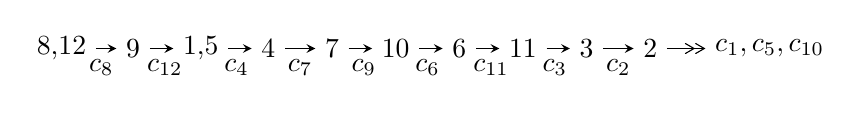
\begin{tikzpicture}[x=23pt, y=7pt]
	% node
	\node (A0) at (-1/8, 0) {8,12};
	\node (A1) at (1, 0) {9};
	\node (A2) at (33/16, 0) {1,5};
	\node (A3) at (25/8, 0) {4};
	\node (A4) at (33/8, 0) {7};
	\node (A5) at (41/8, 0) {10};
	\node (A6) at (49/8, 0) {6};
	\node (A7) at (57/8, 0) {11};
	\node (A8) at (65/8, 0) {3};
	\node (A9) at (73/8, 0) {2};
	\node (C1) at (1/2, -1) {$c_{8}$};
	\node (C2) at (3/2, -1) {$c_{12}$};
	\node (C3) at (21/8, -1) {$c_{4}$};
	\node (C4) at (29/8, -1) {$c_{7}$};
	\node (C5) at (37/8, -1) {$c_{9}$};
	\node (C6) at (45/8, -1) {$c_{6}$};
	\node (C7) at (53/8, -1) {$c_{11}$};
	\node (C8) at (61/8, -1) {$c_{3}$};
	\node (C9) at (69/8, -1) {$c_{2}$};
	\node (A10) at (11, 0) {$c_{1},c_{5},c_{10}$};

	% edge
	\draw[->,>=stealth]	
	(A0) edge (A1) (A1) edge (A2) (A2) edge (A3) (A3) edge (A4) (A4) edge (A5) (A5) edge (A6) (A6) edge (A7) (A7) edge (A8) (A8) edge (A9) ;
	\draw[->>,>={angle 60}]	
	(A9) edge (A10);
\end{tikzpicture} \\ 

\end{tabular} \\

\footnotetext{
The image of knot diagram is generated by the software ``\textbf{Draw programme}" developed by Andrew Bartholomew(\url{http://www.layer8.co.uk/maths/draw/index.htm\#Running-draw}), where we modified some parts for our purpose(\url{https://github.com/CATsTAILs/LinksPainter}).
}\phantom \\ \newline 
\centering \textbf{Ideals for irreducible components\footnotemark of $X_{\text{par}}$} 
 
\begin{align*}
I^u_{1}&=\langle 
-9.26391\times10^{528} u^{121}+1.05469\times10^{529} u^{120}+\cdots+6.31937\times10^{529} b+1.64702\times10^{533},\\
\phantom{I^u_{1}}&\phantom{= \langle  }8.57740\times10^{533} u^{121}-9.52881\times10^{533} u^{120}+\cdots+1.28985\times10^{534} a-1.58398\times10^{538},\\
\phantom{I^u_{1}}&\phantom{= \langle  }u^{122}-46 u^{120}+\cdots-329813 u-20411\rangle \\
I^u_{2}&=\langle 
30599 u^{26}-159948 u^{25}+\cdots+96731 b+60044,\\
\phantom{I^u_{2}}&\phantom{= \langle  }-112679 u^{26}+544868 u^{25}+\cdots+96731 a+61134,\;u^{27}-7 u^{26}+\cdots-3 u+1\rangle \\
\\
\end{align*}
\raggedright * 2 irreducible components of $\dim_{\mathbb{C}}=0$, with total 149 representations.\\
\footnotetext{All coefficients of polynomials are rational numbers. But the coefficients are sometimes approximated in decimal forms when there is not enough margin.}
\newpage
\renewcommand{\arraystretch}{1}
\centering \section*{I. $I^u_{1}= \langle -9.26\times10^{528} u^{121}+1.05\times10^{529} u^{120}+\cdots+6.32\times10^{529} b+1.65\times10^{533},\;8.58\times10^{533} u^{121}-9.53\times10^{533} u^{120}+\cdots+1.29\times10^{534} a-1.58\times10^{538},\;u^{122}-46 u^{120}+\cdots-329813 u-20411 \rangle$}
\flushleft \textbf{(i) Arc colorings}\\
\begin{tabular}{m{7pt} m{180pt} m{7pt} m{180pt} }
\flushright $a_{8}=$&$\begin{pmatrix}1\\0\end{pmatrix}$ \\
\flushright $a_{12}=$&$\begin{pmatrix}0\\u\end{pmatrix}$ \\
\flushright $a_{9}=$&$\begin{pmatrix}1\\- u^2\end{pmatrix}$ \\
\flushright $a_{1}=$&$\begin{pmatrix}u\\- u^3+u\end{pmatrix}$ \\
\flushright $a_{5}=$&$\begin{pmatrix}-0.664993 u^{121}+0.738755 u^{120}+\cdots+187219. u+12280.4\\0.146595 u^{121}-0.166899 u^{120}+\cdots-39879.7 u-2606.30\end{pmatrix}$ \\
\flushright $a_{4}=$&$\begin{pmatrix}-0.518398 u^{121}+0.571856 u^{120}+\cdots+147339. u+9674.07\\0.146595 u^{121}-0.166899 u^{120}+\cdots-39879.7 u-2606.30\end{pmatrix}$ \\
\flushright $a_{7}=$&$\begin{pmatrix}-0.518225 u^{121}+0.534264 u^{120}+\cdots+154724. u+10182.6\\0.0675599 u^{121}-0.0594037 u^{120}+\cdots-22498.9 u-1486.46\end{pmatrix}$ \\
\flushright $a_{10}=$&$\begin{pmatrix}-2.58679 u^{121}+2.79238 u^{120}+\cdots+744064. u+48838.4\\0.486404 u^{121}-0.509217 u^{120}+\cdots-143474. u-9429.90\end{pmatrix}$ \\
\flushright $a_{6}=$&$\begin{pmatrix}-11.6756 u^{121}+12.7481 u^{120}+\cdots+3.32414\times10^{6} u+218060.\\2.38119 u^{121}-2.56874 u^{120}+\cdots-684613. u-44934.0\end{pmatrix}$ \\
\flushright $a_{11}=$&$\begin{pmatrix}-2.51142 u^{121}+2.71118 u^{120}+\cdots+722356. u+47412.4\\0.474861 u^{121}-0.498385 u^{120}+\cdots-139939. u-9198.53\end{pmatrix}$ \\
\flushright $a_{3}=$&$\begin{pmatrix}-2.33035 u^{121}+2.88454 u^{120}+\cdots+581831. u+37845.7\\1.32325 u^{121}-1.52667 u^{120}+\cdots-356834. u-23317.1\end{pmatrix}$ \\
\flushright $a_{2}=$&$\begin{pmatrix}-11.0534 u^{121}+12.1726 u^{120}+\cdots+3.12432\times10^{6} u+204861.\\2.49935 u^{121}-2.76006 u^{120}+\cdots-704365. u-46177.5\end{pmatrix}$\\&\end{tabular}
\flushleft \textbf{(ii) Obstruction class $= -1$}\\~\\
\flushleft \textbf{(iii) Cusp Shapes $= -8.86340 u^{121}+9.44042 u^{120}+\cdots+2.58147\times10^{6} u+169581.$}\\~\\
\newpage\renewcommand{\arraystretch}{1}
\flushleft \textbf{(iv) u-Polynomials at the component}\newline \\
\begin{tabular}{m{50pt}|m{274pt}}
Crossings & \hspace{64pt}u-Polynomials at each crossing \\
\hline $$\begin{aligned}c_{1}\end{aligned}$$&$\begin{aligned}
&u^{122}+54 u^{121}+\cdots+234560 u+3721
\end{aligned}$\\
\hline $$\begin{aligned}c_{2},c_{5}\end{aligned}$$&$\begin{aligned}
&u^{122}+4 u^{121}+\cdots+768 u-61
\end{aligned}$\\
\hline $$\begin{aligned}c_{3},c_{11}\end{aligned}$$&$\begin{aligned}
&u^{122}+u^{121}+\cdots-165778 u+43807
\end{aligned}$\\
\hline $$\begin{aligned}c_{4},c_{7}\end{aligned}$$&$\begin{aligned}
&u^{122}-3 u^{121}+\cdots-48567 u-5581
\end{aligned}$\\
\hline $$\begin{aligned}c_{6},c_{9}\end{aligned}$$&$\begin{aligned}
&u^{122}+11 u^{121}+\cdots+3691 u+583
\end{aligned}$\\
\hline $$\begin{aligned}c_{8},c_{12}\end{aligned}$$&$\begin{aligned}
&u^{122}-46 u^{120}+\cdots+329813 u-20411
\end{aligned}$\\
\hline $$\begin{aligned}c_{10}\end{aligned}$$&$\begin{aligned}
&u^{122}+18 u^{121}+\cdots-1396048 u-97927
\end{aligned}$\\
\hline
\end{tabular}\\~\\
\newpage\renewcommand{\arraystretch}{1}
\flushleft \textbf{(v) Riley Polynomials at the component}\newline \\
\begin{tabular}{m{50pt}|m{274pt}}
Crossings & \hspace{64pt}Riley Polynomials at each crossing \\
\hline $$\begin{aligned}c_{1}\end{aligned}$$&$\begin{aligned}
&y^{122}+42 y^{121}+\cdots-15419630672 y+13845841
\end{aligned}$\\
\hline $$\begin{aligned}c_{2},c_{5}\end{aligned}$$&$\begin{aligned}
&y^{122}-54 y^{121}+\cdots-234560 y+3721
\end{aligned}$\\
\hline $$\begin{aligned}c_{3},c_{11}\end{aligned}$$&$\begin{aligned}
&y^{122}-91 y^{121}+\cdots+72533065960 y+1919053249
\end{aligned}$\\
\hline $$\begin{aligned}c_{4},c_{7}\end{aligned}$$&$\begin{aligned}
&y^{122}+107 y^{121}+\cdots-8059253861 y+31147561
\end{aligned}$\\
\hline $$\begin{aligned}c_{6},c_{9}\end{aligned}$$&$\begin{aligned}
&y^{122}+47 y^{121}+\cdots+16292581 y+339889
\end{aligned}$\\
\hline $$\begin{aligned}c_{8},c_{12}\end{aligned}$$&$\begin{aligned}
&y^{122}-92 y^{121}+\cdots+736931829 y+416608921
\end{aligned}$\\
\hline $$\begin{aligned}c_{10}\end{aligned}$$&$\begin{aligned}
&y^{122}-34 y^{121}+\cdots-80169514796 y+9589697329
\end{aligned}$\\
\hline
\end{tabular}\\~\\
\newpage\flushleft \textbf{(vi) Complex Volumes and Cusp Shapes}
$$\begin{array}{c|c|c}  
\text{Solutions to }I^u_{1}& \I (\text{vol} + \sqrt{-1}CS) & \text{Cusp shape}\\
 \hline 
\begin{aligned}
u &= -0.185283 + 0.995240 I \\
a &= \phantom{-}0.434314 - 0.123749 I \\
b &= \phantom{-}0.083889 + 1.405940 I\end{aligned}
 & \phantom{-}6.74660 - 6.32099 I & \phantom{-0.000000 } 0 \\ \hline\begin{aligned}
u &= -0.185283 - 0.995240 I \\
a &= \phantom{-}0.434314 + 0.123749 I \\
b &= \phantom{-}0.083889 - 1.405940 I\end{aligned}
 & \phantom{-}6.74660 + 6.32099 I & \phantom{-0.000000 } 0 \\ \hline\begin{aligned}
u &= -0.983304 + 0.072186 I \\
a &= -0.186724 - 0.967483 I \\
b &= \phantom{-}0.0603164 - 0.0387061 I\end{aligned}
 & \phantom{-}1.68246 - 2.04205 I & \phantom{-0.000000 } 0 \\ \hline\begin{aligned}
u &= -0.983304 - 0.072186 I \\
a &= -0.186724 + 0.967483 I \\
b &= \phantom{-}0.0603164 + 0.0387061 I\end{aligned}
 & \phantom{-}1.68246 + 2.04205 I & \phantom{-0.000000 } 0 \\ \hline\begin{aligned}
u &= -0.313196 + 0.971427 I \\
a &= \phantom{-}0.265354 + 1.292510 I \\
b &= -0.303709 - 0.441266 I\end{aligned}
 & -4.76986 - 0.10029 I & \phantom{-0.000000 } 0 \\ \hline\begin{aligned}
u &= -0.313196 - 0.971427 I \\
a &= \phantom{-}0.265354 - 1.292510 I \\
b &= -0.303709 + 0.441266 I\end{aligned}
 & -4.76986 + 0.10029 I & \phantom{-0.000000 } 0 \\ \hline\begin{aligned}
u &= \phantom{-}0.919052 + 0.479728 I \\
a &= -0.505013 + 0.467012 I \\
b &= \phantom{-}0.869825 - 0.014469 I\end{aligned}
 & -0.38199 + 2.73563 I & \phantom{-0.000000 } 0 \\ \hline\begin{aligned}
u &= \phantom{-}0.919052 - 0.479728 I \\
a &= -0.505013 - 0.467012 I \\
b &= \phantom{-}0.869825 + 0.014469 I\end{aligned}
 & -0.38199 - 2.73563 I & \phantom{-0.000000 } 0 \\ \hline\begin{aligned}
u &= -1.015850 + 0.256086 I \\
a &= -1.048490 - 0.393541 I \\
b &= -0.229222 - 0.528802 I\end{aligned}
 & \phantom{-}2.53416 + 1.42657 I & \phantom{-0.000000 } 0 \\ \hline\begin{aligned}
u &= -1.015850 - 0.256086 I \\
a &= -1.048490 + 0.393541 I \\
b &= -0.229222 + 0.528802 I\end{aligned}
 & \phantom{-}2.53416 - 1.42657 I & \phantom{-0.000000 } 0\\
 \hline 
 \end{array}$$\newpage$$\begin{array}{c|c|c}  
\text{Solutions to }I^u_{1}& \I (\text{vol} + \sqrt{-1}CS) & \text{Cusp shape}\\
 \hline 
\begin{aligned}
u &= \phantom{-}0.617681 + 0.862562 I \\
a &= -0.158895 - 0.454665 I \\
b &= -0.478962 + 0.583740 I\end{aligned}
 & -5.47979 + 3.39146 I & \phantom{-0.000000 } 0 \\ \hline\begin{aligned}
u &= \phantom{-}0.617681 - 0.862562 I \\
a &= -0.158895 + 0.454665 I \\
b &= -0.478962 - 0.583740 I\end{aligned}
 & -5.47979 - 3.39146 I & \phantom{-0.000000 } 0 \\ \hline\begin{aligned}
u &= -1.094060 + 0.025243 I \\
a &= \phantom{-}1.25305 - 4.74859 I \\
b &= \phantom{-}0.025554 + 1.075220 I\end{aligned}
 & \phantom{-}3.54795 + 1.94440 I & \phantom{-0.000000 } 0 \\ \hline\begin{aligned}
u &= -1.094060 - 0.025243 I \\
a &= \phantom{-}1.25305 + 4.74859 I \\
b &= \phantom{-}0.025554 - 1.075220 I\end{aligned}
 & \phantom{-}3.54795 - 1.94440 I & \phantom{-0.000000 } 0 \\ \hline\begin{aligned}
u &= \phantom{-}0.212618 + 0.880188 I \\
a &= \phantom{-}0.042175 + 1.122760 I \\
b &= -0.442932 - 0.811781 I\end{aligned}
 & -4.92295 - 0.38816 I & \phantom{-0.000000 } 0 \\ \hline\begin{aligned}
u &= \phantom{-}0.212618 - 0.880188 I \\
a &= \phantom{-}0.042175 - 1.122760 I \\
b &= -0.442932 + 0.811781 I\end{aligned}
 & -4.92295 + 0.38816 I & \phantom{-0.000000 } 0 \\ \hline\begin{aligned}
u &= -1.090100 + 0.143218 I \\
a &= \phantom{-}1.99869 - 1.36653 I \\
b &= \phantom{-}0.213229 + 1.033570 I\end{aligned}
 & \phantom{-}3.31035 - 2.58307 I & \phantom{-0.000000 } 0 \\ \hline\begin{aligned}
u &= -1.090100 - 0.143218 I \\
a &= \phantom{-}1.99869 + 1.36653 I \\
b &= \phantom{-}0.213229 - 1.033570 I\end{aligned}
 & \phantom{-}3.31035 + 2.58307 I & \phantom{-0.000000 } 0 \\ \hline\begin{aligned}
u &= -0.254380 + 1.082060 I \\
a &= -0.432421 + 0.207693 I \\
b &= -0.001503 - 1.387090 I\end{aligned}
 & \phantom{-}7.67004 - 0.40713 I & \phantom{-0.000000 } 0 \\ \hline\begin{aligned}
u &= -0.254380 - 1.082060 I \\
a &= -0.432421 - 0.207693 I \\
b &= -0.001503 + 1.387090 I\end{aligned}
 & \phantom{-}7.67004 + 0.40713 I & \phantom{-0.000000 } 0\\
 \hline 
 \end{array}$$\newpage$$\begin{array}{c|c|c}  
\text{Solutions to }I^u_{1}& \I (\text{vol} + \sqrt{-1}CS) & \text{Cusp shape}\\
 \hline 
\begin{aligned}
u &= \phantom{-}1.090430 + 0.258405 I \\
a &= -0.35121 - 1.87368 I \\
b &= \phantom{-}0.26151 + 1.52819 I\end{aligned}
 & \phantom{-}4.83023 - 1.99731 I & \phantom{-0.000000 } 0 \\ \hline\begin{aligned}
u &= \phantom{-}1.090430 - 0.258405 I \\
a &= -0.35121 + 1.87368 I \\
b &= \phantom{-}0.26151 - 1.52819 I\end{aligned}
 & \phantom{-}4.83023 + 1.99731 I & \phantom{-0.000000 } 0 \\ \hline\begin{aligned}
u &= \phantom{-}1.001540 + 0.527659 I \\
a &= \phantom{-}0.587001 - 0.336708 I \\
b &= -0.884271 - 0.193902 I\end{aligned}
 & -1.57250 + 7.74927 I & \phantom{-0.000000 } 0 \\ \hline\begin{aligned}
u &= \phantom{-}1.001540 - 0.527659 I \\
a &= \phantom{-}0.587001 + 0.336708 I \\
b &= -0.884271 + 0.193902 I\end{aligned}
 & -1.57250 - 7.74927 I & \phantom{-0.000000 } 0 \\ \hline\begin{aligned}
u &= -1.130960 + 0.223715 I \\
a &= \phantom{-}0.53891 - 1.92792 I \\
b &= \phantom{-}0.62911 + 2.00733 I\end{aligned}
 & \phantom{-}9.17958 - 4.12880 I & \phantom{-0.000000 } 0 \\ \hline\begin{aligned}
u &= -1.130960 - 0.223715 I \\
a &= \phantom{-}0.53891 + 1.92792 I \\
b &= \phantom{-}0.62911 - 2.00733 I\end{aligned}
 & \phantom{-}9.17958 + 4.12880 I & \phantom{-0.000000 } 0 \\ \hline\begin{aligned}
u &= -1.125760 + 0.253622 I \\
a &= \phantom{-}0.511983 - 0.428645 I \\
b &= \phantom{-}0.758439 + 0.708769 I\end{aligned}
 & \phantom{-}3.64396 - 3.00386 I & \phantom{-0.000000 } 0 \\ \hline\begin{aligned}
u &= -1.125760 - 0.253622 I \\
a &= \phantom{-}0.511983 + 0.428645 I \\
b &= \phantom{-}0.758439 - 0.708769 I\end{aligned}
 & \phantom{-}3.64396 + 3.00386 I & \phantom{-0.000000 } 0 \\ \hline\begin{aligned}
u &= -1.138500 + 0.248182 I \\
a &= -0.75065 + 1.90644 I \\
b &= -0.35236 - 2.00818 I\end{aligned}
 & \phantom{-}9.07248 + 1.65253 I & \phantom{-0.000000 } 0 \\ \hline\begin{aligned}
u &= -1.138500 - 0.248182 I \\
a &= -0.75065 - 1.90644 I \\
b &= -0.35236 + 2.00818 I\end{aligned}
 & \phantom{-}9.07248 - 1.65253 I & \phantom{-0.000000 } 0\\
 \hline 
 \end{array}$$\newpage$$\begin{array}{c|c|c}  
\text{Solutions to }I^u_{1}& \I (\text{vol} + \sqrt{-1}CS) & \text{Cusp shape}\\
 \hline 
\begin{aligned}
u &= \phantom{-}0.963772 + 0.735482 I \\
a &= \phantom{-}0.348408 + 0.019050 I \\
b &= -0.319827 - 0.365548 I\end{aligned}
 & -4.51317 + 2.35259 I & \phantom{-0.000000 } 0 \\ \hline\begin{aligned}
u &= \phantom{-}0.963772 - 0.735482 I \\
a &= \phantom{-}0.348408 - 0.019050 I \\
b &= -0.319827 + 0.365548 I\end{aligned}
 & -4.51317 - 2.35259 I & \phantom{-0.000000 } 0 \\ \hline\begin{aligned}
u &= \phantom{-}1.187670 + 0.257386 I \\
a &= \phantom{-}0.23652 + 1.93229 I \\
b &= \phantom{-}0.00178 - 1.56169 I\end{aligned}
 & \phantom{-}5.58538 + 3.88018 I & \phantom{-0.000000 } 0 \\ \hline\begin{aligned}
u &= \phantom{-}1.187670 - 0.257386 I \\
a &= \phantom{-}0.23652 - 1.93229 I \\
b &= \phantom{-}0.00178 + 1.56169 I\end{aligned}
 & \phantom{-}5.58538 - 3.88018 I & \phantom{-0.000000 } 0 \\ \hline\begin{aligned}
u &= -1.224900 + 0.132148 I \\
a &= -0.73527 + 1.92025 I \\
b &= -0.024419 - 1.313570 I\end{aligned}
 & \phantom{-}4.60074 + 0.06454 I & \phantom{-0.000000 } 0 \\ \hline\begin{aligned}
u &= -1.224900 - 0.132148 I \\
a &= -0.73527 - 1.92025 I \\
b &= -0.024419 + 1.313570 I\end{aligned}
 & \phantom{-}4.60074 - 0.06454 I & \phantom{-0.000000 } 0 \\ \hline\begin{aligned}
u &= \phantom{-}0.349897 + 0.670589 I \\
a &= -0.298869 - 0.710686 I \\
b &= -0.780936 + 0.454130 I\end{aligned}
 & -3.40658 - 3.29129 I & \phantom{-0.000000 } 0 \\ \hline\begin{aligned}
u &= \phantom{-}0.349897 - 0.670589 I \\
a &= -0.298869 + 0.710686 I \\
b &= -0.780936 - 0.454130 I\end{aligned}
 & -3.40658 + 3.29129 I & \phantom{-0.000000 } 0 \\ \hline\begin{aligned}
u &= -1.232020 + 0.242519 I \\
a &= -0.458416 - 0.297642 I \\
b &= \phantom{-}1.54582 + 0.35213 I\end{aligned}
 & \phantom{-}4.28648 - 5.49663 I & \phantom{-0.000000 } 0 \\ \hline\begin{aligned}
u &= -1.232020 - 0.242519 I \\
a &= -0.458416 + 0.297642 I \\
b &= \phantom{-}1.54582 - 0.35213 I\end{aligned}
 & \phantom{-}4.28648 + 5.49663 I & \phantom{-0.000000 } 0\\
 \hline 
 \end{array}$$\newpage$$\begin{array}{c|c|c}  
\text{Solutions to }I^u_{1}& \I (\text{vol} + \sqrt{-1}CS) & \text{Cusp shape}\\
 \hline 
\begin{aligned}
u &= \phantom{-}0.103548 + 0.733188 I \\
a &= -0.319880 + 0.705862 I \\
b &= -0.611185 - 1.009860 I\end{aligned}
 & -1.77326 - 8.36598 I & \phantom{-0.000000 } 0 \\ \hline\begin{aligned}
u &= \phantom{-}0.103548 - 0.733188 I \\
a &= -0.319880 - 0.705862 I \\
b &= -0.611185 + 1.009860 I\end{aligned}
 & -1.77326 + 8.36598 I & \phantom{-0.000000 } 0 \\ \hline\begin{aligned}
u &= \phantom{-}0.508711 + 0.517972 I \\
a &= \phantom{-}0.020939 + 0.810543 I \\
b &= \phantom{-}0.702476 - 0.389803 I\end{aligned}
 & -1.55574 + 1.18943 I & \phantom{-0.000000 } 0 \\ \hline\begin{aligned}
u &= \phantom{-}0.508711 - 0.517972 I \\
a &= \phantom{-}0.020939 - 0.810543 I \\
b &= \phantom{-}0.702476 + 0.389803 I\end{aligned}
 & -1.55574 - 1.18943 I & \phantom{-0.000000 } 0 \\ \hline\begin{aligned}
u &= -1.259230 + 0.239950 I \\
a &= \phantom{-}0.605728 + 0.167825 I \\
b &= -1.66675 - 0.17193 I\end{aligned}
 & \phantom{-}2.77395 - 11.03740 I & \phantom{-0.000000 } 0 \\ \hline\begin{aligned}
u &= -1.259230 - 0.239950 I \\
a &= \phantom{-}0.605728 - 0.167825 I \\
b &= -1.66675 + 0.17193 I\end{aligned}
 & \phantom{-}2.77395 + 11.03740 I & \phantom{-0.000000 } 0 \\ \hline\begin{aligned}
u &= \phantom{-}1.28424\phantom{ +0.000000I} \\
a &= -0.182483\phantom{ +0.000000I} \\
b &= \phantom{-}1.09077\phantom{ +0.000000I}\end{aligned}
 & \phantom{-}2.33642\phantom{ +0.000000I} & \phantom{-0.000000 } 0 \\ \hline\begin{aligned}
u &= -1.242320 + 0.327818 I \\
a &= \phantom{-}0.206622 - 0.146648 I \\
b &= -1.129820 + 0.001367 I\end{aligned}
 & -1.50052 - 4.11143 I & \phantom{-0.000000 } 0 \\ \hline\begin{aligned}
u &= -1.242320 - 0.327818 I \\
a &= \phantom{-}0.206622 + 0.146648 I \\
b &= -1.129820 - 0.001367 I\end{aligned}
 & -1.50052 + 4.11143 I & \phantom{-0.000000 } 0 \\ \hline\begin{aligned}
u &= \phantom{-}1.256120 + 0.328598 I \\
a &= -0.08162 - 2.02613 I \\
b &= -0.191382 + 1.230830 I\end{aligned}
 & -1.42430 + 4.48045 I & \phantom{-0.000000 } 0\\
 \hline 
 \end{array}$$\newpage$$\begin{array}{c|c|c}  
\text{Solutions to }I^u_{1}& \I (\text{vol} + \sqrt{-1}CS) & \text{Cusp shape}\\
 \hline 
\begin{aligned}
u &= \phantom{-}1.256120 - 0.328598 I \\
a &= -0.08162 + 2.02613 I \\
b &= -0.191382 - 1.230830 I\end{aligned}
 & -1.42430 - 4.48045 I & \phantom{-0.000000 } 0 \\ \hline\begin{aligned}
u &= \phantom{-}0.111179 + 0.690149 I \\
a &= \phantom{-}0.082288 - 0.622290 I \\
b &= \phantom{-}0.505590 + 1.004630 I\end{aligned}
 & \phantom{-}0.24654 - 3.21510 I & \phantom{-0.000000 } 0 \\ \hline\begin{aligned}
u &= \phantom{-}0.111179 - 0.690149 I \\
a &= \phantom{-}0.082288 + 0.622290 I \\
b &= \phantom{-}0.505590 - 1.004630 I\end{aligned}
 & \phantom{-}0.24654 + 3.21510 I & \phantom{-0.000000 } 0 \\ \hline\begin{aligned}
u &= \phantom{-}1.264340 + 0.323180 I \\
a &= -0.24787 - 2.17167 I \\
b &= -0.377052 + 1.263140 I\end{aligned}
 & \phantom{-}1.89644 + 12.20220 I & \phantom{-0.000000 } 0 \\ \hline\begin{aligned}
u &= \phantom{-}1.264340 - 0.323180 I \\
a &= -0.24787 + 2.17167 I \\
b &= -0.377052 - 1.263140 I\end{aligned}
 & \phantom{-}1.89644 - 12.20220 I & \phantom{-0.000000 } 0 \\ \hline\begin{aligned}
u &= \phantom{-}1.266750 + 0.316138 I \\
a &= \phantom{-}0.24407 + 2.07352 I \\
b &= \phantom{-}0.332473 - 1.326910 I\end{aligned}
 & \phantom{-}3.91879 + 6.93656 I & \phantom{-0.000000 } 0 \\ \hline\begin{aligned}
u &= \phantom{-}1.266750 - 0.316138 I \\
a &= \phantom{-}0.24407 - 2.07352 I \\
b &= \phantom{-}0.332473 + 1.326910 I\end{aligned}
 & \phantom{-}3.91879 - 6.93656 I & \phantom{-0.000000 } 0 \\ \hline\begin{aligned}
u &= -0.334371 + 0.565524 I \\
a &= -0.793853 - 0.739199 I \\
b &= -0.388025 - 0.836475 I\end{aligned}
 & \phantom{-}1.55438 - 0.12200 I & \phantom{-0.000000 } 0 \\ \hline\begin{aligned}
u &= -0.334371 - 0.565524 I \\
a &= -0.793853 + 0.739199 I \\
b &= -0.388025 + 0.836475 I\end{aligned}
 & \phantom{-}1.55438 + 0.12200 I & \phantom{-0.000000 } 0 \\ \hline\begin{aligned}
u &= -0.368653 + 0.542730 I \\
a &= -0.587831 - 1.011260 I \\
b &= -0.397710 - 1.137590 I\end{aligned}
 & \phantom{-}2.42769 - 3.87191 I & \phantom{-0.000000 } 0\\
 \hline 
 \end{array}$$\newpage$$\begin{array}{c|c|c}  
\text{Solutions to }I^u_{1}& \I (\text{vol} + \sqrt{-1}CS) & \text{Cusp shape}\\
 \hline 
\begin{aligned}
u &= -0.368653 - 0.542730 I \\
a &= -0.587831 + 1.011260 I \\
b &= -0.397710 + 1.137590 I\end{aligned}
 & \phantom{-}2.42769 + 3.87191 I & \phantom{-0.000000 } 0 \\ \hline\begin{aligned}
u &= -1.337120 + 0.155962 I \\
a &= -0.54295 + 1.62380 I \\
b &= \phantom{-}0.264196 - 1.340780 I\end{aligned}
 & \phantom{-}5.05912 + 0.47037 I & \phantom{-0.000000 } 0 \\ \hline\begin{aligned}
u &= -1.337120 - 0.155962 I \\
a &= -0.54295 - 1.62380 I \\
b &= \phantom{-}0.264196 + 1.340780 I\end{aligned}
 & \phantom{-}5.05912 - 0.47037 I & \phantom{-0.000000 } 0 \\ \hline\begin{aligned}
u &= -0.295131 + 0.581464 I \\
a &= -0.85667 - 1.84488 I \\
b &= \phantom{-}0.619427 + 0.073935 I\end{aligned}
 & \phantom{-}1.23260 + 2.48040 I & \phantom{-0.000000 } 0 \\ \hline\begin{aligned}
u &= -0.295131 - 0.581464 I \\
a &= -0.85667 + 1.84488 I \\
b &= \phantom{-}0.619427 - 0.073935 I\end{aligned}
 & \phantom{-}1.23260 - 2.48040 I & \phantom{-0.000000 } 0 \\ \hline\begin{aligned}
u &= -0.411888 + 0.504365 I \\
a &= -1.018360 - 0.680281 I \\
b &= -0.067693 - 0.513016 I\end{aligned}
 & \phantom{-}1.72082 - 0.02250 I & \phantom{-0.000000 } 0 \\ \hline\begin{aligned}
u &= -0.411888 - 0.504365 I \\
a &= -1.018360 + 0.680281 I \\
b &= -0.067693 + 0.513016 I\end{aligned}
 & \phantom{-}1.72082 + 0.02250 I & \phantom{-0.000000 } 0 \\ \hline\begin{aligned}
u &= -0.649192\phantom{ +0.000000I} \\
a &= -0.589360\phantom{ +0.000000I} \\
b &= -0.0907688\phantom{ +0.000000I}\end{aligned}
 & \phantom{-}0.892793\phantom{ +0.000000I} & \phantom{-}12.3040\phantom{ +0.000000I} \\ \hline\begin{aligned}
u &= -0.169610 + 0.622301 I \\
a &= \phantom{-}0.200395 + 0.225308 I \\
b &= \phantom{-}0.268657 + 1.102790 I\end{aligned}
 & \phantom{-}1.38119 - 2.52030 I & \phantom{-0.000000 } 0 \\ \hline\begin{aligned}
u &= -0.169610 - 0.622301 I \\
a &= \phantom{-}0.200395 - 0.225308 I \\
b &= \phantom{-}0.268657 - 1.102790 I\end{aligned}
 & \phantom{-}1.38119 + 2.52030 I & \phantom{-0.000000 } 0\\
 \hline 
 \end{array}$$\newpage$$\begin{array}{c|c|c}  
\text{Solutions to }I^u_{1}& \I (\text{vol} + \sqrt{-1}CS) & \text{Cusp shape}\\
 \hline 
\begin{aligned}
u &= -1.355990 + 0.008881 I \\
a &= \phantom{-}0.13469 + 1.59361 I \\
b &= -0.226282 - 0.916721 I\end{aligned}
 & \phantom{-}2.13275 + 1.36234 I & \phantom{-0.000000 } 0 \\ \hline\begin{aligned}
u &= -1.355990 - 0.008881 I \\
a &= \phantom{-}0.13469 - 1.59361 I \\
b &= -0.226282 + 0.916721 I\end{aligned}
 & \phantom{-}2.13275 - 1.36234 I & \phantom{-0.000000 } 0 \\ \hline\begin{aligned}
u &= \phantom{-}1.363310 + 0.033367 I \\
a &= -0.261013 - 0.342681 I \\
b &= -0.787977 + 0.235223 I\end{aligned}
 & \phantom{-}7.61827 + 1.39910 I & \phantom{-0.000000 } 0 \\ \hline\begin{aligned}
u &= \phantom{-}1.363310 - 0.033367 I \\
a &= -0.261013 + 0.342681 I \\
b &= -0.787977 - 0.235223 I\end{aligned}
 & \phantom{-}7.61827 - 1.39910 I & \phantom{-0.000000 } 0 \\ \hline\begin{aligned}
u &= \phantom{-}1.371890 + 0.093794 I \\
a &= \phantom{-}0.046962 + 0.650836 I \\
b &= \phantom{-}0.949159 - 0.481079 I\end{aligned}
 & \phantom{-}5.89354 + 6.46464 I & \phantom{-0.000000 } 0 \\ \hline\begin{aligned}
u &= \phantom{-}1.371890 - 0.093794 I \\
a &= \phantom{-}0.046962 - 0.650836 I \\
b &= \phantom{-}0.949159 + 0.481079 I\end{aligned}
 & \phantom{-}5.89354 - 6.46464 I & \phantom{-0.000000 } 0 \\ \hline\begin{aligned}
u &= -0.369828 + 0.501185 I \\
a &= \phantom{-}0.444203 + 1.090710 I \\
b &= \phantom{-}0.316244 + 1.163110 I\end{aligned}
 & \phantom{-}2.53576 + 0.53218 I & \phantom{-0.000000 } 0 \\ \hline\begin{aligned}
u &= -0.369828 - 0.501185 I \\
a &= \phantom{-}0.444203 - 1.090710 I \\
b &= \phantom{-}0.316244 - 1.163110 I\end{aligned}
 & \phantom{-}2.53576 - 0.53218 I & \phantom{-0.000000 } 0 \\ \hline\begin{aligned}
u &= -0.197740 + 0.567124 I \\
a &= \phantom{-}0.56110 + 2.24172 I \\
b &= -0.750285 - 0.179233 I\end{aligned}
 & -0.65485 + 8.09028 I & \phantom{-0.000000 } 0 \\ \hline\begin{aligned}
u &= -0.197740 - 0.567124 I \\
a &= \phantom{-}0.56110 - 2.24172 I \\
b &= -0.750285 + 0.179233 I\end{aligned}
 & -0.65485 - 8.09028 I & \phantom{-0.000000 } 0\\
 \hline 
 \end{array}$$\newpage$$\begin{array}{c|c|c}  
\text{Solutions to }I^u_{1}& \I (\text{vol} + \sqrt{-1}CS) & \text{Cusp shape}\\
 \hline 
\begin{aligned}
u &= \phantom{-}0.150836 + 1.400180 I \\
a &= \phantom{-}0.015381 - 0.345136 I \\
b &= -0.306678 + 1.297390 I\end{aligned}
 & \phantom{-}3.07475 + 11.83000 I & \phantom{-0.000000 } 0 \\ \hline\begin{aligned}
u &= \phantom{-}0.150836 - 1.400180 I \\
a &= \phantom{-}0.015381 + 0.345136 I \\
b &= -0.306678 - 1.297390 I\end{aligned}
 & \phantom{-}3.07475 - 11.83000 I & \phantom{-0.000000 } 0 \\ \hline\begin{aligned}
u &= \phantom{-}1.40556 + 0.20546 I \\
a &= -0.03983 + 1.65725 I \\
b &= \phantom{-}0.92844 - 1.70992 I\end{aligned}
 & \phantom{-}8.11081 + 2.07745 I & \phantom{-0.000000 } 0 \\ \hline\begin{aligned}
u &= \phantom{-}1.40556 - 0.20546 I \\
a &= -0.03983 - 1.65725 I \\
b &= \phantom{-}0.92844 + 1.70992 I\end{aligned}
 & \phantom{-}8.11081 - 2.07745 I & \phantom{-0.000000 } 0 \\ \hline\begin{aligned}
u &= -0.250777 + 0.512072 I \\
a &= \phantom{-}0.949567 + 0.809716 I \\
b &= \phantom{-}0.566377 + 0.438121 I\end{aligned}
 & \phantom{-}0.67353 - 4.33386 I & \phantom{-0.000000 -}0. + 7.02296 I \\ \hline\begin{aligned}
u &= -0.250777 - 0.512072 I \\
a &= \phantom{-}0.949567 - 0.809716 I \\
b &= \phantom{-}0.566377 - 0.438121 I\end{aligned}
 & \phantom{-}0.67353 + 4.33386 I & \phantom{-0.000000 } 0. - 7.02296 I \\ \hline\begin{aligned}
u &= \phantom{-}1.41554 + 0.20667 I \\
a &= \phantom{-}0.09786 - 1.59194 I \\
b &= -1.05602 + 1.64043 I\end{aligned}
 & \phantom{-}8.08886 + 6.60048 I & \phantom{-0.000000 } 0 \\ \hline\begin{aligned}
u &= \phantom{-}1.41554 - 0.20667 I \\
a &= \phantom{-}0.09786 + 1.59194 I \\
b &= -1.05602 - 1.64043 I\end{aligned}
 & \phantom{-}8.08886 - 6.60048 I & \phantom{-0.000000 } 0 \\ \hline\begin{aligned}
u &= -1.42157 + 0.16278 I \\
a &= \phantom{-}0.45715 - 1.43573 I \\
b &= -0.456912 + 1.245300 I\end{aligned}
 & \phantom{-}3.42642 + 5.06397 I & \phantom{-0.000000 } 0 \\ \hline\begin{aligned}
u &= -1.42157 - 0.16278 I \\
a &= \phantom{-}0.45715 + 1.43573 I \\
b &= -0.456912 - 1.245300 I\end{aligned}
 & \phantom{-}3.42642 - 5.06397 I & \phantom{-0.000000 } 0\\
 \hline 
 \end{array}$$\newpage$$\begin{array}{c|c|c}  
\text{Solutions to }I^u_{1}& \I (\text{vol} + \sqrt{-1}CS) & \text{Cusp shape}\\
 \hline 
\begin{aligned}
u &= \phantom{-}1.42549 + 0.20836 I \\
a &= \phantom{-}0.046821 - 1.369870 I \\
b &= -1.04513 + 1.30066 I\end{aligned}
 & \phantom{-}7.21313 + 2.93325 I & \phantom{-0.000000 } 0 \\ \hline\begin{aligned}
u &= \phantom{-}1.42549 - 0.20836 I \\
a &= \phantom{-}0.046821 + 1.369870 I \\
b &= -1.04513 - 1.30066 I\end{aligned}
 & \phantom{-}7.21313 - 2.93325 I & \phantom{-0.000000 } 0 \\ \hline\begin{aligned}
u &= \phantom{-}1.42185 + 0.28595 I \\
a &= \phantom{-}0.32402 + 1.54579 I \\
b &= \phantom{-}0.60512 - 1.41033 I\end{aligned}
 & \phantom{-}6.52707 + 5.96383 I & \phantom{-0.000000 } 0 \\ \hline\begin{aligned}
u &= \phantom{-}1.42185 - 0.28595 I \\
a &= \phantom{-}0.32402 - 1.54579 I \\
b &= \phantom{-}0.60512 + 1.41033 I\end{aligned}
 & \phantom{-}6.52707 - 5.96383 I & \phantom{-0.000000 } 0 \\ \hline\begin{aligned}
u &= \phantom{-}0.04806 + 1.46007 I \\
a &= -0.087709 + 0.373885 I \\
b &= \phantom{-}0.231939 - 1.312120 I\end{aligned}
 & \phantom{-}5.26484 + 5.45539 I & \phantom{-0.000000 } 0 \\ \hline\begin{aligned}
u &= \phantom{-}0.04806 - 1.46007 I \\
a &= -0.087709 - 0.373885 I \\
b &= \phantom{-}0.231939 + 1.312120 I\end{aligned}
 & \phantom{-}5.26484 - 5.45539 I & \phantom{-0.000000 } 0 \\ \hline\begin{aligned}
u &= \phantom{-}1.41517 + 0.44626 I \\
a &= \phantom{-}0.76965 + 1.47422 I \\
b &= \phantom{-}0.42129 - 1.46978 I\end{aligned}
 & \phantom{-}11.7726 + 11.4995 I & \phantom{-0.000000 } 0 \\ \hline\begin{aligned}
u &= \phantom{-}1.41517 - 0.44626 I \\
a &= \phantom{-}0.76965 - 1.47422 I \\
b &= \phantom{-}0.42129 + 1.46978 I\end{aligned}
 & \phantom{-}11.7726 - 11.4995 I & \phantom{-0.000000 } 0 \\ \hline\begin{aligned}
u &= \phantom{-}1.44834 + 0.45505 I \\
a &= -0.73719 - 1.38855 I \\
b &= -0.38461 + 1.43888 I\end{aligned}
 & \phantom{-}13.0030 + 5.8555 I & \phantom{-0.000000 } 0 \\ \hline\begin{aligned}
u &= \phantom{-}1.44834 - 0.45505 I \\
a &= -0.73719 + 1.38855 I \\
b &= -0.38461 - 1.43888 I\end{aligned}
 & \phantom{-}13.0030 - 5.8555 I & \phantom{-0.000000 } 0\\
 \hline 
 \end{array}$$\newpage$$\begin{array}{c|c|c}  
\text{Solutions to }I^u_{1}& \I (\text{vol} + \sqrt{-1}CS) & \text{Cusp shape}\\
 \hline 
\begin{aligned}
u &= -1.28455 + 0.88465 I \\
a &= -0.665983 + 1.094100 I \\
b &= -0.09402 - 1.51647 I\end{aligned}
 & \phantom{-}9.30469 + 0.14343 I & \phantom{-0.000000 } 0 \\ \hline\begin{aligned}
u &= -1.28455 - 0.88465 I \\
a &= -0.665983 - 1.094100 I \\
b &= -0.09402 + 1.51647 I\end{aligned}
 & \phantom{-}9.30469 - 0.14343 I & \phantom{-0.000000 } 0 \\ \hline\begin{aligned}
u &= -1.51320 + 0.55870 I \\
a &= -0.42687 + 1.51074 I \\
b &= -0.59681 - 1.56994 I\end{aligned}
 & \phantom{-}8.4055 - 18.5940 I & \phantom{-0.000000 } 0 \\ \hline\begin{aligned}
u &= -1.51320 - 0.55870 I \\
a &= -0.42687 - 1.51074 I \\
b &= -0.59681 + 1.56994 I\end{aligned}
 & \phantom{-}8.4055 + 18.5940 I & \phantom{-0.000000 } 0 \\ \hline\begin{aligned}
u &= \phantom{-}1.61043 + 0.18462 I \\
a &= \phantom{-}0.388375 + 1.179820 I \\
b &= \phantom{-}0.462835 - 1.035540 I\end{aligned}
 & \phantom{-}6.15338 + 6.15152 I & \phantom{-0.000000 } 0 \\ \hline\begin{aligned}
u &= \phantom{-}1.61043 - 0.18462 I \\
a &= \phantom{-}0.388375 - 1.179820 I \\
b &= \phantom{-}0.462835 + 1.035540 I\end{aligned}
 & \phantom{-}6.15338 - 6.15152 I & \phantom{-0.000000 } 0 \\ \hline\begin{aligned}
u &= -1.51451 + 0.58350 I \\
a &= \phantom{-}0.44911 - 1.47326 I \\
b &= \phantom{-}0.53582 + 1.57275 I\end{aligned}
 & \phantom{-}10.3791 - 12.5012 I & \phantom{-0.000000 } 0 \\ \hline\begin{aligned}
u &= -1.51451 - 0.58350 I \\
a &= \phantom{-}0.44911 + 1.47326 I \\
b &= \phantom{-}0.53582 - 1.57275 I\end{aligned}
 & \phantom{-}10.3791 + 12.5012 I & \phantom{-0.000000 } 0 \\ \hline\begin{aligned}
u &= -1.45381 + 0.76710 I \\
a &= \phantom{-}0.559538 - 1.257950 I \\
b &= \phantom{-}0.25618 + 1.54059 I\end{aligned}
 & \phantom{-}10.80050 - 6.60908 I & \phantom{-0.000000 } 0 \\ \hline\begin{aligned}
u &= -1.45381 - 0.76710 I \\
a &= \phantom{-}0.559538 + 1.257950 I \\
b &= \phantom{-}0.25618 - 1.54059 I\end{aligned}
 & \phantom{-}10.80050 + 6.60908 I & \phantom{-0.000000 } 0\\
 \hline 
 \end{array}$$\newpage$$\begin{array}{c|c|c}  
\text{Solutions to }I^u_{1}& \I (\text{vol} + \sqrt{-1}CS) & \text{Cusp shape}\\
 \hline 
\begin{aligned}
u &= \phantom{-}0.043376 + 0.317650 I \\
a &= \phantom{-}0.86810 + 1.34327 I \\
b &= \phantom{-}0.541558 - 0.138767 I\end{aligned}
 & -1.34088 + 0.49926 I & -5.57781 - 0.86695 I \\ \hline\begin{aligned}
u &= \phantom{-}0.043376 - 0.317650 I \\
a &= \phantom{-}0.86810 - 1.34327 I \\
b &= \phantom{-}0.541558 + 0.138767 I\end{aligned}
 & -1.34088 - 0.49926 I & -5.57781 + 0.86695 I \\ \hline\begin{aligned}
u &= -1.60710 + 0.61679 I \\
a &= -0.37388 + 1.37210 I \\
b &= -0.46338 - 1.43070 I\end{aligned}
 & \phantom{-}3.25452 - 9.72714 I & \phantom{-0.000000 } 0 \\ \hline\begin{aligned}
u &= -1.60710 - 0.61679 I \\
a &= -0.37388 - 1.37210 I \\
b &= -0.46338 + 1.43070 I\end{aligned}
 & \phantom{-}3.25452 + 9.72714 I & \phantom{-0.000000 } 0 \\ \hline\begin{aligned}
u &= -0.246391 + 0.118040 I \\
a &= -0.57374 + 2.30124 I \\
b &= \phantom{-}0.066255 + 1.006660 I\end{aligned}
 & \phantom{-}2.27701 - 2.35404 I & \phantom{-}1.13682 + 3.61254 I \\ \hline\begin{aligned}
u &= -0.246391 - 0.118040 I \\
a &= -0.57374 - 2.30124 I \\
b &= \phantom{-}0.066255 - 1.006660 I\end{aligned}
 & \phantom{-}2.27701 + 2.35404 I & \phantom{-}1.13682 - 3.61254 I \\ \hline\begin{aligned}
u &= \phantom{-}1.65253 + 0.51466 I \\
a &= -0.576270 - 1.116790 I \\
b &= -0.244766 + 1.249460 I\end{aligned}
 & \phantom{-}10.77680 + 2.11340 I & \phantom{-0.000000 } 0 \\ \hline\begin{aligned}
u &= \phantom{-}1.65253 - 0.51466 I \\
a &= -0.576270 + 1.116790 I \\
b &= -0.244766 - 1.249460 I\end{aligned}
 & \phantom{-}10.77680 - 2.11340 I & \phantom{-0.000000 } 0 \\ \hline\begin{aligned}
u &= \phantom{-}1.71930 + 0.68117 I \\
a &= \phantom{-}0.550280 + 0.982535 I \\
b &= \phantom{-}0.142931 - 1.206000 I\end{aligned}
 & \phantom{-}7.79971 - 3.82442 I & \phantom{-0.000000 } 0 \\ \hline\begin{aligned}
u &= \phantom{-}1.71930 - 0.68117 I \\
a &= \phantom{-}0.550280 - 0.982535 I \\
b &= \phantom{-}0.142931 + 1.206000 I\end{aligned}
 & \phantom{-}7.79971 + 3.82442 I & \phantom{-0.000000 } 0\\
 \hline 
 \end{array}$$\newpage$$\begin{array}{c|c|c}  
\text{Solutions to }I^u_{1}& \I (\text{vol} + \sqrt{-1}CS) & \text{Cusp shape}\\
 \hline 
\begin{aligned}
u &= -0.24042 + 1.84495 I \\
a &= \phantom{-}0.171420 - 0.573839 I \\
b &= -0.105804 + 1.247870 I\end{aligned}
 & -1.97749 + 1.23305 I & \phantom{-0.000000 } 0 \\ \hline\begin{aligned}
u &= -0.24042 - 1.84495 I \\
a &= \phantom{-}0.171420 + 0.573839 I \\
b &= -0.105804 - 1.247870 I\end{aligned}
 & -1.97749 - 1.23305 I & \phantom{-0.000000 } 0\\
 \hline 
 \end{array}$$\newpage\newpage\renewcommand{\arraystretch}{1}
\centering \section*{II. $I^u_{2}= \langle 30599 u^{26}-159948 u^{25}+\cdots+96731 b+60044,\;-1.13\times10^{5} u^{26}+5.45\times10^{5} u^{25}+\cdots+9.67\times10^{4} a+6.11\times10^{4},\;u^{27}-7 u^{26}+\cdots-3 u+1 \rangle$}
\flushleft \textbf{(i) Arc colorings}\\
\begin{tabular}{m{7pt} m{180pt} m{7pt} m{180pt} }
\flushright $a_{8}=$&$\begin{pmatrix}1\\0\end{pmatrix}$ \\
\flushright $a_{12}=$&$\begin{pmatrix}0\\u\end{pmatrix}$ \\
\flushright $a_{9}=$&$\begin{pmatrix}1\\- u^2\end{pmatrix}$ \\
\flushright $a_{1}=$&$\begin{pmatrix}u\\- u^3+u\end{pmatrix}$ \\
\flushright $a_{5}=$&$\begin{pmatrix}1.16487 u^{26}-5.63282 u^{25}+\cdots+7.47333 u-0.632000\\-0.316331 u^{26}+1.65353 u^{25}+\cdots-0.183943 u-0.620732\end{pmatrix}$ \\
\flushright $a_{4}=$&$\begin{pmatrix}0.848539 u^{26}-3.97928 u^{25}+\cdots+7.28939 u-1.25273\\-0.316331 u^{26}+1.65353 u^{25}+\cdots-0.183943 u-0.620732\end{pmatrix}$ \\
\flushright $a_{7}=$&$\begin{pmatrix}-1.51963 u^{26}+10.0236 u^{25}+\cdots-3.78453 u+4.65857\\0.613816 u^{26}-3.83224 u^{25}+\cdots+3.90031 u-1.51963\end{pmatrix}$ \\
\flushright $a_{10}=$&$\begin{pmatrix}7.85801 u^{26}-65.4779 u^{25}+\cdots-39.8520 u+8.37763\\-0.149342 u^{26}+2.78904 u^{25}+\cdots-0.578491 u+0.905811\end{pmatrix}$ \\
\flushright $a_{6}=$&$\begin{pmatrix}6.42087 u^{26}-53.2276 u^{25}+\cdots+1.62778 u+2.55334\\-6.96505 u^{26}+55.7644 u^{25}+\cdots+34.4717 u-9.63398\end{pmatrix}$ \\
\flushright $a_{11}=$&$\begin{pmatrix}8.85801 u^{26}-71.4779 u^{25}+\cdots-36.8520 u+7.37763\\-0.149342 u^{26}+2.78904 u^{25}+\cdots+0.421509 u+0.905811\end{pmatrix}$ \\
\flushright $a_{3}=$&$\begin{pmatrix}12.7463 u^{26}-100.682 u^{25}+\cdots-51.5229 u+13.9725\\0.600645 u^{26}-5.22174 u^{25}+\cdots+2.66461 u-1.80247\end{pmatrix}$ \\
\flushright $a_{2}=$&$\begin{pmatrix}-12.3296 u^{26}+100.395 u^{25}+\cdots+55.1362 u-12.2366\\1.98117 u^{26}-17.3079 u^{25}+\cdots+7.14347 u-2.42784\end{pmatrix}$\\&\end{tabular}
\flushleft \textbf{(ii) Obstruction class $= 1$}\\~\\
\flushleft \textbf{(iii) Cusp Shapes $= -\frac{3441662}{96731} u^{26}+\frac{26608834}{96731} u^{25}+\cdots+\frac{13611309}{96731} u-\frac{2509628}{96731}$}\\~\\
\newpage\renewcommand{\arraystretch}{1}
\flushleft \textbf{(iv) u-Polynomials at the component}\newline \\
\begin{tabular}{m{50pt}|m{274pt}}
Crossings & \hspace{64pt}u-Polynomials at each crossing \\
\hline $$\begin{aligned}c_{1}\end{aligned}$$&$\begin{aligned}
&u^{27}-17 u^{26}+\cdots+16 u-1
\end{aligned}$\\
\hline $$\begin{aligned}c_{2}\end{aligned}$$&$\begin{aligned}
&u^{27}+3 u^{26}+\cdots-6 u-1
\end{aligned}$\\
\hline $$\begin{aligned}c_{3}\end{aligned}$$&$\begin{aligned}
&u^{27}-2 u^{26}+\cdots+2 u-1
\end{aligned}$\\
\hline $$\begin{aligned}c_{4}\end{aligned}$$&$\begin{aligned}
&u^{27}-2 u^{26}+\cdots-9 u-1
\end{aligned}$\\
\hline $$\begin{aligned}c_{5}\end{aligned}$$&$\begin{aligned}
&u^{27}-3 u^{26}+\cdots-6 u+1
\end{aligned}$\\
\hline $$\begin{aligned}c_{6}\end{aligned}$$&$\begin{aligned}
&u^{27}+2 u^{26}+\cdots- u+1
\end{aligned}$\\
\hline $$\begin{aligned}c_{7}\end{aligned}$$&$\begin{aligned}
&u^{27}+2 u^{26}+\cdots-9 u+1
\end{aligned}$\\
\hline $$\begin{aligned}c_{8}\end{aligned}$$&$\begin{aligned}
&u^{27}-7 u^{26}+\cdots-3 u+1
\end{aligned}$\\
\hline $$\begin{aligned}c_{9}\end{aligned}$$&$\begin{aligned}
&u^{27}-2 u^{26}+\cdots- u-1
\end{aligned}$\\
\hline $$\begin{aligned}c_{10}\end{aligned}$$&$\begin{aligned}
&u^{27}+u^{26}+\cdots+20 u+1
\end{aligned}$\\
\hline $$\begin{aligned}c_{11}\end{aligned}$$&$\begin{aligned}
&u^{27}+2 u^{26}+\cdots+2 u+1
\end{aligned}$\\
\hline $$\begin{aligned}c_{12}\end{aligned}$$&$\begin{aligned}
&u^{27}+7 u^{26}+\cdots-3 u-1
\end{aligned}$\\
\hline
\end{tabular}\\~\\
\newpage\renewcommand{\arraystretch}{1}
\flushleft \textbf{(v) Riley Polynomials at the component}\newline \\
\begin{tabular}{m{50pt}|m{274pt}}
Crossings & \hspace{64pt}Riley Polynomials at each crossing \\
\hline $$\begin{aligned}c_{1}\end{aligned}$$&$\begin{aligned}
&y^{27}- y^{26}+\cdots-88 y-1
\end{aligned}$\\
\hline $$\begin{aligned}c_{2},c_{5}\end{aligned}$$&$\begin{aligned}
&y^{27}-17 y^{26}+\cdots+16 y-1
\end{aligned}$\\
\hline $$\begin{aligned}c_{3},c_{11}\end{aligned}$$&$\begin{aligned}
&y^{27}-6 y^{26}+\cdots+298 y^2-1
\end{aligned}$\\
\hline $$\begin{aligned}c_{4},c_{7}\end{aligned}$$&$\begin{aligned}
&y^{27}+28 y^{26}+\cdots+45 y-1
\end{aligned}$\\
\hline $$\begin{aligned}c_{6},c_{9}\end{aligned}$$&$\begin{aligned}
&y^{27}-8 y^{25}+\cdots-5 y-1
\end{aligned}$\\
\hline $$\begin{aligned}c_{8},c_{12}\end{aligned}$$&$\begin{aligned}
&y^{27}-15 y^{26}+\cdots+3 y-1
\end{aligned}$\\
\hline $$\begin{aligned}c_{10}\end{aligned}$$&$\begin{aligned}
&y^{27}-9 y^{26}+\cdots+28 y-1
\end{aligned}$\\
\hline
\end{tabular}\\~\\
\newpage\flushleft \textbf{(vi) Complex Volumes and Cusp Shapes}
$$\begin{array}{c|c|c}  
\text{Solutions to }I^u_{2}& \I (\text{vol} + \sqrt{-1}CS) & \text{Cusp shape}\\
 \hline 
\begin{aligned}
u &= -0.107787 + 1.060130 I \\
a &= -0.26125 + 1.39730 I \\
b &= \phantom{-}0.255392 - 0.708618 I\end{aligned}
 & -4.36986 + 0.94186 I & \phantom{-}4.32882 - 7.97316 I \\ \hline\begin{aligned}
u &= -0.107787 - 1.060130 I \\
a &= -0.26125 - 1.39730 I \\
b &= \phantom{-}0.255392 + 0.708618 I\end{aligned}
 & -4.36986 - 0.94186 I & \phantom{-}4.32882 + 7.97316 I \\ \hline\begin{aligned}
u &= \phantom{-}0.876248 + 0.702233 I \\
a &= -0.376364 - 0.135976 I \\
b &= \phantom{-}0.193817 - 0.009805 I\end{aligned}
 & -4.54338 + 2.71100 I & \phantom{-}0.44164 - 10.63785 I \\ \hline\begin{aligned}
u &= \phantom{-}0.876248 - 0.702233 I \\
a &= -0.376364 + 0.135976 I \\
b &= \phantom{-}0.193817 + 0.009805 I\end{aligned}
 & -4.54338 - 2.71100 I & \phantom{-}0.44164 + 10.63785 I \\ \hline\begin{aligned}
u &= -1.160540 + 0.048438 I \\
a &= \phantom{-}0.04155 - 1.92162 I \\
b &= -0.17288 + 1.43623 I\end{aligned}
 & \phantom{-}5.04480 + 2.65528 I & \phantom{-}5.96897 - 5.01438 I \\ \hline\begin{aligned}
u &= -1.160540 - 0.048438 I \\
a &= \phantom{-}0.04155 + 1.92162 I \\
b &= -0.17288 - 1.43623 I\end{aligned}
 & \phantom{-}5.04480 - 2.65528 I & \phantom{-}5.96897 + 5.01438 I \\ \hline\begin{aligned}
u &= -1.163620 + 0.040576 I \\
a &= -0.78576 + 3.19152 I \\
b &= -0.029594 - 1.086680 I\end{aligned}
 & \phantom{-}3.65676 + 1.89859 I & \phantom{-}16.5619 + 2.3505 I \\ \hline\begin{aligned}
u &= -1.163620 - 0.040576 I \\
a &= -0.78576 - 3.19152 I \\
b &= -0.029594 + 1.086680 I\end{aligned}
 & \phantom{-}3.65676 - 1.89859 I & \phantom{-}16.5619 - 2.3505 I \\ \hline\begin{aligned}
u &= -0.801697\phantom{ +0.000000I} \\
a &= \phantom{-}0.269073\phantom{ +0.000000I} \\
b &= -0.565798\phantom{ +0.000000I}\end{aligned}
 & \phantom{-}0.124792\phantom{ +0.000000I} & -0.864170\phantom{ +0.000000I} \\ \hline\begin{aligned}
u &= -0.785361 + 0.062897 I \\
a &= -0.79466 - 1.35040 I \\
b &= -0.060019 - 0.874276 I\end{aligned}
 & \phantom{-}2.82979 - 2.23758 I & \phantom{-}22.0223 - 3.8705 I\\
 \hline 
 \end{array}$$\newpage$$\begin{array}{c|c|c}  
\text{Solutions to }I^u_{2}& \I (\text{vol} + \sqrt{-1}CS) & \text{Cusp shape}\\
 \hline 
\begin{aligned}
u &= -0.785361 - 0.062897 I \\
a &= -0.79466 + 1.35040 I \\
b &= -0.060019 + 0.874276 I\end{aligned}
 & \phantom{-}2.82979 + 2.23758 I & \phantom{-}22.0223 + 3.8705 I \\ \hline\begin{aligned}
u &= \phantom{-}1.211370 + 0.581494 I \\
a &= \phantom{-}0.65438 + 1.46116 I \\
b &= \phantom{-}0.23699 - 1.78233 I\end{aligned}
 & \phantom{-}8.33811 - 0.73456 I & \phantom{-}3.49155 + 0. I\phantom{ +0.000000I} \\ \hline\begin{aligned}
u &= \phantom{-}1.211370 - 0.581494 I \\
a &= \phantom{-}0.65438 - 1.46116 I \\
b &= \phantom{-}0.23699 + 1.78233 I\end{aligned}
 & \phantom{-}8.33811 + 0.73456 I & \phantom{-}3.49155 + 0. I\phantom{ +0.000000I} \\ \hline\begin{aligned}
u &= \phantom{-}1.294820 + 0.370255 I \\
a &= -0.31810 - 1.70609 I \\
b &= -0.65325 + 1.85007 I\end{aligned}
 & \phantom{-}9.19948 + 5.20084 I & \phantom{-}8.18979 - 5.87227 I \\ \hline\begin{aligned}
u &= \phantom{-}1.294820 - 0.370255 I \\
a &= -0.31810 + 1.70609 I \\
b &= -0.65325 - 1.85007 I\end{aligned}
 & \phantom{-}9.19948 - 5.20084 I & \phantom{-}8.18979 + 5.87227 I \\ \hline\begin{aligned}
u &= \phantom{-}0.534303 + 0.368722 I \\
a &= -2.08988 + 0.61152 I \\
b &= \phantom{-}0.617007 - 0.425699 I\end{aligned}
 & \phantom{-}0.22469 + 9.10529 I & \phantom{-}4.87426 - 8.12456 I \\ \hline\begin{aligned}
u &= \phantom{-}0.534303 - 0.368722 I \\
a &= -2.08988 - 0.61152 I \\
b &= \phantom{-}0.617007 + 0.425699 I\end{aligned}
 & \phantom{-}0.22469 - 9.10529 I & \phantom{-}4.87426 + 8.12456 I \\ \hline\begin{aligned}
u &= \phantom{-}1.41158 + 0.15557 I \\
a &= \phantom{-}0.06103 - 1.46451 I \\
b &= -1.02813 + 1.36328 I\end{aligned}
 & \phantom{-}7.39362 + 3.73716 I & \phantom{-}7.16285 - 6.64593 I \\ \hline\begin{aligned}
u &= \phantom{-}1.41158 - 0.15557 I \\
a &= \phantom{-}0.06103 + 1.46451 I \\
b &= -1.02813 - 1.36328 I\end{aligned}
 & \phantom{-}7.39362 - 3.73716 I & \phantom{-}7.16285 + 6.64593 I \\ \hline\begin{aligned}
u &= \phantom{-}0.350268 + 0.334731 I \\
a &= \phantom{-}2.29916 - 1.47517 I \\
b &= -0.579949 + 0.586242 I\end{aligned}
 & \phantom{-}1.91007 + 3.52122 I & \phantom{-}7.19053 - 4.22290 I\\
 \hline 
 \end{array}$$\newpage$$\begin{array}{c|c|c}  
\text{Solutions to }I^u_{2}& \I (\text{vol} + \sqrt{-1}CS) & \text{Cusp shape}\\
 \hline 
\begin{aligned}
u &= \phantom{-}0.350268 - 0.334731 I \\
a &= \phantom{-}2.29916 + 1.47517 I \\
b &= -0.579949 - 0.586242 I\end{aligned}
 & \phantom{-}1.91007 - 3.52122 I & \phantom{-}7.19053 + 4.22290 I \\ \hline\begin{aligned}
u &= -0.164164 + 0.382515 I \\
a &= -0.44634 - 1.60994 I \\
b &= -0.375995 - 1.017170 I\end{aligned}
 & \phantom{-}1.92294 - 1.73525 I & \phantom{-}4.59316 + 1.63174 I \\ \hline\begin{aligned}
u &= -0.164164 - 0.382515 I \\
a &= -0.44634 + 1.60994 I \\
b &= -0.375995 + 1.017170 I\end{aligned}
 & \phantom{-}1.92294 + 1.73525 I & \phantom{-}4.59316 - 1.63174 I \\ \hline\begin{aligned}
u &= -0.01422 + 1.60586 I \\
a &= -0.151767 - 0.443205 I \\
b &= \phantom{-}0.142590 + 1.192110 I\end{aligned}
 & -2.46276 - 0.55570 I & \phantom{-0.000000 } 0 \\ \hline\begin{aligned}
u &= -0.01422 - 1.60586 I \\
a &= -0.151767 + 0.443205 I \\
b &= \phantom{-}0.142590 - 1.192110 I\end{aligned}
 & -2.46276 + 0.55570 I & \phantom{-0.000000 } 0 \\ \hline\begin{aligned}
u &= \phantom{-}1.61796 + 0.10292 I \\
a &= \phantom{-}0.033471 + 1.305770 I \\
b &= \phantom{-}0.736915 - 1.144590 I\end{aligned}
 & \phantom{-}5.33696 + 7.15481 I & \phantom{-0.000000 } 0. - 7.70887 I \\ \hline\begin{aligned}
u &= \phantom{-}1.61796 - 0.10292 I \\
a &= \phantom{-}0.033471 - 1.305770 I \\
b &= \phantom{-}0.736915 + 1.144590 I\end{aligned}
 & \phantom{-}5.33696 - 7.15481 I & \phantom{-0.000000 -}0. + 7.70887 I\\
 \hline 
 \end{array}$$\newpage
\newpage\renewcommand{\arraystretch}{1}
\centering \section*{ III. u-Polynomials}
\begin{tabular}{m{50pt}|m{274pt}}
Crossings & \hspace{64pt}u-Polynomials at each crossing \\
\hline $$\begin{aligned}c_{1}\end{aligned}$$&$\begin{aligned}
&(u^{27}-17 u^{26}+\cdots+16 u-1)(u^{122}+54 u^{121}+\cdots+234560 u+3721)
\end{aligned}$\\
\hline $$\begin{aligned}c_{2}\end{aligned}$$&$\begin{aligned}
&(u^{27}+3 u^{26}+\cdots-6 u-1)(u^{122}+4 u^{121}+\cdots+768 u-61)
\end{aligned}$\\
\hline $$\begin{aligned}c_{3}\end{aligned}$$&$\begin{aligned}
&(u^{27}-2 u^{26}+\cdots+2 u-1)(u^{122}+u^{121}+\cdots-165778 u+43807)
\end{aligned}$\\
\hline $$\begin{aligned}c_{4}\end{aligned}$$&$\begin{aligned}
&(u^{27}-2 u^{26}+\cdots-9 u-1)(u^{122}-3 u^{121}+\cdots-48567 u-5581)
\end{aligned}$\\
\hline $$\begin{aligned}c_{5}\end{aligned}$$&$\begin{aligned}
&(u^{27}-3 u^{26}+\cdots-6 u+1)(u^{122}+4 u^{121}+\cdots+768 u-61)
\end{aligned}$\\
\hline $$\begin{aligned}c_{6}\end{aligned}$$&$\begin{aligned}
&(u^{27}+2 u^{26}+\cdots- u+1)(u^{122}+11 u^{121}+\cdots+3691 u+583)
\end{aligned}$\\
\hline $$\begin{aligned}c_{7}\end{aligned}$$&$\begin{aligned}
&(u^{27}+2 u^{26}+\cdots-9 u+1)(u^{122}-3 u^{121}+\cdots-48567 u-5581)
\end{aligned}$\\
\hline $$\begin{aligned}c_{8}\end{aligned}$$&$\begin{aligned}
&(u^{27}-7 u^{26}+\cdots-3 u+1)(u^{122}-46 u^{120}+\cdots+329813 u-20411)
\end{aligned}$\\
\hline $$\begin{aligned}c_{9}\end{aligned}$$&$\begin{aligned}
&(u^{27}-2 u^{26}+\cdots- u-1)(u^{122}+11 u^{121}+\cdots+3691 u+583)
\end{aligned}$\\
\hline $$\begin{aligned}c_{10}\end{aligned}$$&$\begin{aligned}
&(u^{27}+u^{26}+\cdots+20 u+1)(u^{122}+18 u^{121}+\cdots-1396048 u-97927)
\end{aligned}$\\
\hline $$\begin{aligned}c_{11}\end{aligned}$$&$\begin{aligned}
&(u^{27}+2 u^{26}+\cdots+2 u+1)(u^{122}+u^{121}+\cdots-165778 u+43807)
\end{aligned}$\\
\hline $$\begin{aligned}c_{12}\end{aligned}$$&$\begin{aligned}
&(u^{27}+7 u^{26}+\cdots-3 u-1)(u^{122}-46 u^{120}+\cdots+329813 u-20411)
\end{aligned}$\\
\hline
\end{tabular}\newpage\renewcommand{\arraystretch}{1}
\centering \section*{ IV. Riley Polynomials}
\begin{tabular}{m{50pt}|m{274pt}}
Crossings & \hspace{64pt}Riley Polynomials at each crossing \\
\hline $$\begin{aligned}c_{1}\end{aligned}$$&$\begin{aligned}
&(y^{27}- y^{26}+\cdots-88 y-1)\\
&\cdot(y^{122}+42 y^{121}+\cdots-15419630672 y+13845841)
\end{aligned}$\\
\hline $$\begin{aligned}c_{2},c_{5}\end{aligned}$$&$\begin{aligned}
&(y^{27}-17 y^{26}+\cdots+16 y-1)(y^{122}-54 y^{121}+\cdots-234560 y+3721)
\end{aligned}$\\
\hline $$\begin{aligned}c_{3},c_{11}\end{aligned}$$&$\begin{aligned}
&(y^{27}-6 y^{26}+\cdots+298 y^2-1)\\
&\cdot(y^{122}-91 y^{121}+\cdots+72533065960 y+1919053249)
\end{aligned}$\\
\hline $$\begin{aligned}c_{4},c_{7}\end{aligned}$$&$\begin{aligned}
&(y^{27}+28 y^{26}+\cdots+45 y-1)\\
&\cdot(y^{122}+107 y^{121}+\cdots-8059253861 y+31147561)
\end{aligned}$\\
\hline $$\begin{aligned}c_{6},c_{9}\end{aligned}$$&$\begin{aligned}
&(y^{27}-8 y^{25}+\cdots-5 y-1)\\
&\cdot(y^{122}+47 y^{121}+\cdots+16292581 y+339889)
\end{aligned}$\\
\hline $$\begin{aligned}c_{8},c_{12}\end{aligned}$$&$\begin{aligned}
&(y^{27}-15 y^{26}+\cdots+3 y-1)\\
&\cdot(y^{122}-92 y^{121}+\cdots+736931829 y+416608921)
\end{aligned}$\\
\hline $$\begin{aligned}c_{10}\end{aligned}$$&$\begin{aligned}
&(y^{27}-9 y^{26}+\cdots+28 y-1)\\
&\cdot(y^{122}-34 y^{121}+\cdots-80169514796 y+9589697329)
\end{aligned}$\\
\hline
\end{tabular}
\vskip 2pc
\end{document}